\documentclass[final,a4paper,openany,12pt]{mwbk}
%\documentclass[final,a4paper,openright,12pt]{mwbk} % każdy rozdział zaczyna się na stronie nieparzystej
\usepackage{polski}
\usepackage[utf8]{inputenc}
\usepackage{fancyhdr}
\usepackage{url}
\usepackage{algorithm}
\usepackage{algpseudocode}
\usepackage{enumerate}
\usepackage{subcaption}
\captionsetup{compatibility=false}
\usepackage{titlesec}
\usepackage{amsmath}
\usepackage{listings}
\lstset{
language=Python,
breaklines=true,
tabsize=2,
breaklines  = true,
breakatwhitespace   = false,
prebreak= \space,
postbreak   = \space  
}   



\titleformat{\section}[runin]
{\normalfont\Large\bfseries}{\thesection}{1em}{}
\titleformat{\subsection}[runin]
{\normalfont\large\bfseries}{\thesubsection}{1em}{}




\usepackage{makeidx}  % allows index generation
\usepackage{graphicx} % standard LaTeX graphics tool
                      % for including eps-figure files
\graphicspath{{img/}{img/Zegarek}}
\usepackage{float}


%\prefixing %polskie znaki: /a /c /e /z /x /o /s /l /A /C itd. %ZAKOMENTOWANE BO SIE NIE DA UZYWAC "/"

\renewcommand*\listalgorithmname{Spis algorytmów\protect} % łatka na niedoróbkę w spisie algorytmów - nie usuwać!

% zestaw przydatny, kiedy trzeba regulować szerokość kolumn w tablicy:
%%\usepackage{longtable}
%\usepackage{array}
%\newcolumntype{L}[1]{>{\raggedright\let\newline\\\arraybackslash\hspace{0pt}}m{#1}}
%\newcolumntype{C}[1]{>{\centering\let\newline\\\arraybackslash\hspace{0pt}}m{#1}}
%\newcolumntype{R}[1]{>{\raggedleft\let\newline\\\arraybackslash\hspace{0pt}}m{#1}}

\newtheorem{twr}{Twierdzenie}[section]

% ustawienia do wydruku dwustronnego z uwzględnieniem dodatkowego miejsca na zszycie
\setlength{\oddsidemargin}{0.46cm}   %margines nieparzysty
\setlength{\evensidemargin}{-0.54cm} %margines parzysty
\setlength{\textwidth}{16cm}         %szerokość tekstu na stronie
\linespread{1.1}    % lekkie zwiększenie odstępu między liniami, żeby tekst nie był taki ścisły, ponieważ
                    % Odstęp pojedynczej interlinii nie jest komfortowy, kiedy trzeba czytać strony A4
% koniec ustawień

%\makeindex            % used for the subject index
                      % please use the style sprmidx.sty with
                      % your makeindex program
\begin{document}

\begin{titlepage}
\vspace{-0.5cm}

{\centering
{\footnotesize
\begin{tabular}{c}
UNIWERSYTET KARDYNAŁA STEFANA WYSZYŃSKIEGO\\
W WARSZAWIE\\
\end{tabular}
}
\vspace{2.5cm}

{\footnotesize
\begin{tabular}{c}
WYDZIAŁ MATEMATYCZNO-PRZYRODNICZY\\
SZKOŁA NAUK ŚCISŁYCH\\
\end{tabular}
}
\vspace{2.5cm}

\renewcommand{\arraystretch}{1.5} % zwiększamy odległość między wierszami

{\normalsize
\begin{tabular}{c}
Katarzyna Mitrus\\
Michał Słotwiński\\
\end{tabular}
}

\vspace{1.5cm}

{\large
\begin{tabular}{c}

Wprowadzenie do Przetwarzania Obrazów\\
Sprawozdanie z laboratorium\\

\end{tabular}
}

}

\renewcommand{\arraystretch}{1} % przywracamy domyślną odległość miedzy wierszami

\vspace{5cm}

\hspace{6cm}
\begin{tabular}{l}
Prowadzący:\\
prof. Wojciech Mokrzycki\\

\end{tabular}

\vspace{4cm}

{\centering

{\small
\begin{tabular}{c}
{Warszawa, 2018}\\
\end{tabular}
}

}
\end{titlepage}

\tableofcontents
\listoffigures
%\listoftables
%\listofalgorithms

\sloppy


\chapter {Wstęp}

Laboratoria oh oh...~\cite{BookMok} %przynajmniej jedna cytacja dla kompilatora LATEX


\section {Specyfikacja wykorzystanego fortmatu obrazu}

\section {Intstrukcja obsługi programu}



\chapter{Operacje ujednolicania obrazów}
1. ujednolicenie obrazów szarych geometryczne (liczba wierszy i kolumn piksli)
2. ujednolicenie obrazów szarych rozdzielczościowe (w rastrze)
3. ujednolicenie obrazów RGB geometryczne (liczba wierszy i kolumn piksli)
4. ujednolicenie obrazów RGB rozdzielczościowe (w rastrze)

\chapter{Operacje sumowania arytmetycznego obrazów szarych}

Arytmetyczne operacje między pikslami $p$ i $q$ dwóch obrazów są używane w wielu działach przetwarzania obrazów. Przeprowadzane się je wykonując działania na pojedynczych pikslach i są uwarunkowane wymaganiami zależnymi od typu operacji. 
Po operacjach arytmetycznych zwykle niezbędna jest normalizacja. W przedstawionych zadaniach do normalizacji wykorzystano wzór:
	
	\begin{center}
		$ f_{norm} = Z_{rep}[(f - f_{min}) / (f_{max} - f_{min})] $
	\end{center}

\section {Sumowanie (określonej) stałej z obrazem oraz dwóch obrazów}
%\subsection*{Opis algorytmu}
\hfill
\\\\
\indent
Algorytm sumowania obrazu szarego z określoną stałą polega na dodaniu do każdej wartości pojedynczego piksla stałej liczby.
Po operacji sumowania następuje normalizacja obrazu.

	\begin{enumerate}	
		\item Policz sumy wartości kazdego piksla ze stałą ($const$).
		\item Jeżeli jedna z tych sum jest większa niż 255 to:
		\item Wybierz największą sumę  $Q_{max}$ i policz $D_{max}$ ze wzoru: $D_{max}[i,j] = (Q_{max}[i,j] - 255)$ 
		\item Oblicz $X = D_{max} / 255$
		\item Policz sumy ze wzoru
		\begin{center}$Q[i,j] = P[i,j] - (P[i,j]* X) + const - (const * X) $ \\

		\end{center}
	\end{enumerate}

\begin{figure}[H]
	\begin{center}
		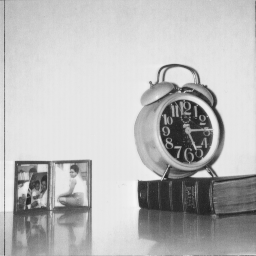
\includegraphics[width=0.3\textwidth]{1/1Gray_Const_Sum_Original}
		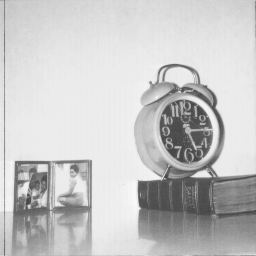
\includegraphics[width=0.3\textwidth]{1/1Gray_Const_Sum_Result}
		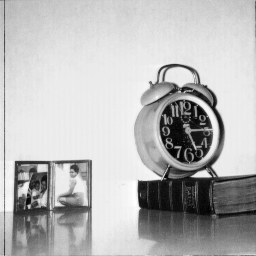
\includegraphics[width=0.3\textwidth]{1/1Gray_Const_Sum_Result_Norm}
	\end{center}
	\caption{Od lewej obraz wejściowy, obraz po sumowaniu ze stałą = 50, obraz po normalizacji }
\end{figure}

\begin{figure}[H]
	\begin{center}
		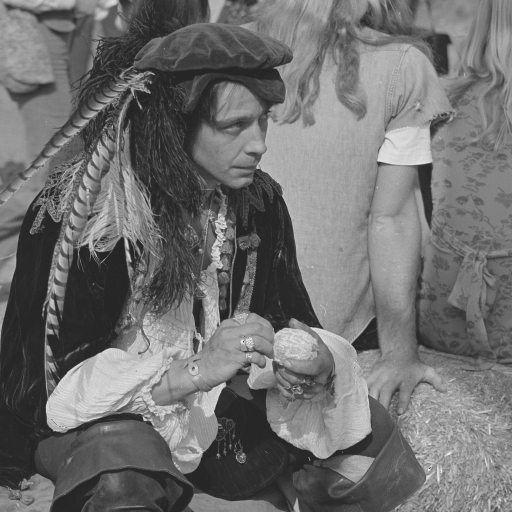
\includegraphics[width=0.3\textwidth]{2/2Gray_Const_Sum_Original}
		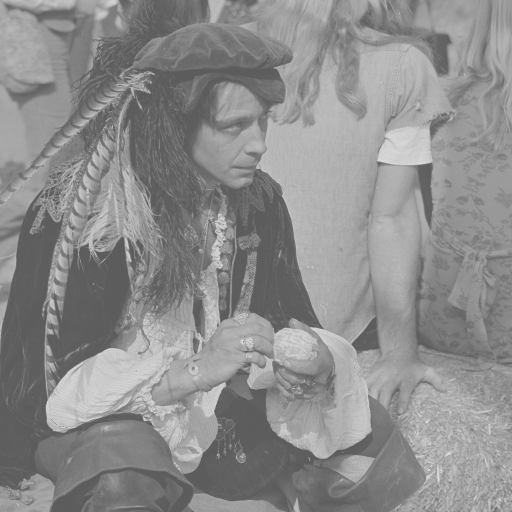
\includegraphics[width=0.3\textwidth]{2/2Gray_Const_Sum_Result}
		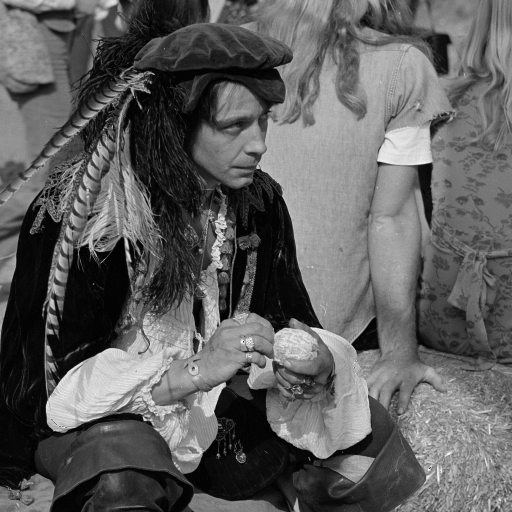
\includegraphics[width=0.3\textwidth]{2/2Gray_Const_Sum_Result_Norm}
	\end{center}
	\caption{Od lewej obraz wejściowy, obraz po sumowaniu ze stałą = 100, obraz po normalizacji }
\end{figure}


\begin{lstlisting}[caption=Sumowanie obrazu ze stałą]

image_matrix = self.im1
width = image_matrix.shape[1]    # szereoksc
height = image_matrix.shape[0]   # wysokosc

result_matrix = np.zeros((width, height), dtype=np.uint8)

# Inicjalizacja zmiennych
Q_max = 0
D_max = 0
X = 0
f_min = 255
f_max = 0

for y in range(height):
    for x in range(width):  
        # Obliczanie sumy
        L = int(image_matrix[x][y]) + int(const)

        # Poszukiwanie maksimum
        if Q_max < L:
            Q_max = L

# Sprawdzenie czy przekracza zakres
if Q_max > 255:
    D_max = Q_max - 255
    X = (D_max/255)

# Obliczenie sumy z uwzglednieniem zakresu
for y in range(height):
    for x in range(width): 
        L = (image_matrix[x][y] - (image_matrix[x][y] * X)) + (const - (const * X))

        # Zaokroglenie do najblizszej wartosci calkowitej z gory
        # i przypisanie wartosci
        result_matrix[x][y] = math.ceil(L)

        # Poszukiwanie minimum i maksimum
        if f_min > L:
            f_min = L
        if f_max < L:
            f_max = L
\end{lstlisting}





\section {Mnożenie obrazu przez zadaną liczbę oraz przez inny obraz}
\section {Mieszanie obrazów z określonym współczynnikiem}
\section {Potęgowanie obrazu (z zadaną potęgą)}
\section {Dzielenie obrazu przez (zadaną) liczbę oraz przez inny obraz}
\section {Pierwiastkowanie obrazu}
\section {Logarytmowanie obrazu}

\chapter{Operacje sumowania arytmetycznego obrazów barwowych}
1. sumowanie (określonej) stałej z obrazem oraz dwóch obrazów
2. mnożenie obrazu przez zadaną liczbę oraz przez inny obraz
3. mieszanie obrazów z określonym współczynnikiem
4. potęgowanie obrazu (z zadaną potęgą)
5. dzielenie obrazu przez (zadaną) liczbę oraz przez inny obraz
6. pierwiastkowanie obrazu
7. logarytmowanie obrazu

\chapter{Operacje geometryczne na obrazie}
1. przemieszczenie obrazu o zadany wektor
2. jednorodne i niejednorodne skalowanie obrazu
3. obracanie obrazu o dowolny kąt
4. symetrie względem osi układu i zadanej prostej
5. wycinanie fragmentów obrazu
6. kopiowanie fragmentów obrazów

\chapter{Operacje na histogramie obrazu szarego}
1. obliczanie histogramu
2. przemieszczanie histogramu
3. rozciąganie histogramu
4. progowanie lokalne
5. progowanie globalne

\chapter{Operacje na histogramie obrazu barwowego}
1. obliczanie histogramu
2. przemieszczanie histogramu
3. rozciąganie histogramu
4. progowanie 1-progowe
5. progowanie wieloprogowe
6. progowanie lokalne
7. progowanie globalne

\chapter{Operacje morfologiczne na obrazach binarnych}
1. okrawanie(erozja)
2. nakładanie (dylatacja)
3. otwarcie
4. zamknięcie

\chapter {Operacje morfologiczne na obrazach szarych}
1. okrawanie(erozja)
2. nakładanie (dylatacja)
3. otwarcie
4. zamknięcie

\chapter {Filtrowanie liniowe i nieliniowe}
1. dolnoprzepustowe (dwa do wyboru)
2. górnoprzepustowe (Robertsa, Prewitta, Sobela, ....)
3. gradientowe (kompasowe, płaskorzeźbowe kierunkowe, gradientu wektorowego VGO, gradientu
wektora kierunkowego VDG).
4. medianowe
5. ekstremalne

\chapter{Podsumowanie}

Lorem ipsum dolor sit amet, consectetur adipiscing elit, sed do eiusmod tempor incididunt ut labore et dolore magna aliqua. Ut enim ad minim veniam, quis nostrud exercitation ullamco laboris nisi ut aliquip ex ea commodo consequat. Duis aute irure dolor in reprehenderit in voluptate velit esse cillum dolore eu fugiat nulla pariatur. Excepteur sint occaecat cupidatat non proident, sunt in culpa qui officia deserunt mollit anim id est laborum.

\bibliographystyle{plain}
\bibliography{literatura}

\end{document} 